\documentclass{article}
\usepackage[utf8]{inputenc}

\title{Astronomy 121 Lab 2: Digital Electronics}
\author{Vikram Iyer}
\date{\today}

\usepackage{natbib}
\usepackage{graphicx}
\usepackage{listings}
\usepackage[margin=1.0in]{geometry}


\begin{document}

\maketitle

%=======================================================================================

\begin{abstract}
\end{abstract}

%=======================================================================================
%Need
% sun and moon diameter
% least squares plot for each
% 1 hour sun plot
% horizon to horizon sun, filtered
% moon plot, spectrum, filtered
% point source plot, spectrum, filtered
% expected fringe frequencies eq11

% rotation matrices
11GHz, small sources
all info is in f, amp, phase of fringe
Baseline = 10m
fringe spacing \frac{\lambda}{B}
multiplying => 2E_1E_2

need precessed ra and dec

use UTC to find sidereal time at Long 0deg (HMS), RA tells what part of sky is
overhead

Use your long oto calcultae offset and find LST

RA-LST = HA (hour angle)
use lat and

state rotation matrices, explain procedure

Fringe F depends on  cos(\delta)

Formula in lab document is for east west baseline (approx correct for this
interferometer)

Fringe amplitude vs

interf output = cycles/hr

Finding frequency
Make a guess at value of $\frac{B_y}{\lambda}\cos \delta$
Pick a value for RA to get h from LST
Least squares with amplitude
Save R^2, continue for different guesses, find min
with A and B of min, calculate cable length \tau_c

total delay
$$\Tau_{tot}=\Tau_{g}(h_s)+\Tau_c$$
$\Tau_g$ is the geometric path delay between the two telescopes and is a
function of time, the hour angle of the source $h_s$
$\Tau_c$ is the delay in the cable which will be determined using least-squares.


\section{Introduction}
Interferometry is a common tool in radio astronomy both for the purpose of
correlating multiple signals to improve the signal to noise ratio (SNR)
of weak astronomical signals, as well as to improve the resolution with which
one can observe the sky. The purpose of this lab experiment was to learn and
apply the basic principles of interferometry to measure the diameter of the sun
and the moon, as well as the baseline length of the interferometer from the
known declination of a point source. After recording and processing the raw data
we applied least squares to obtain a function of best fit to the processed data in order to determine the quantities of interest such as source diameter and
baseline.
%=======================================================================================
%lstinline
%citep
\section{Methods}
  \subsection{Interferometer}
  The interferometer consists of two 1m diameter dishes along an approximately
  10m East-West baseline. Each antenna output is connected to a series of analog
  filters and amplifiers prior to sampling.  After initial amplification and
  filtering at the source of the signal, the inputs are down converted from an
  original frequency of 10.7 GHz. This output is down converted again and
  filtered to a bandwidth of 30MHz. The outputs of the two dishes are then mixed
  and sampled.  The data is collected by an HP digital voltmeter connected via
  GPIB to a Linux workstation. This computer is capable of both recording the
  output as well as controlling the motors to point the telescope. The full
  signal path is shown in \ref{fig:signal_path}.

    \begin{figure}[h!]
    \centering
    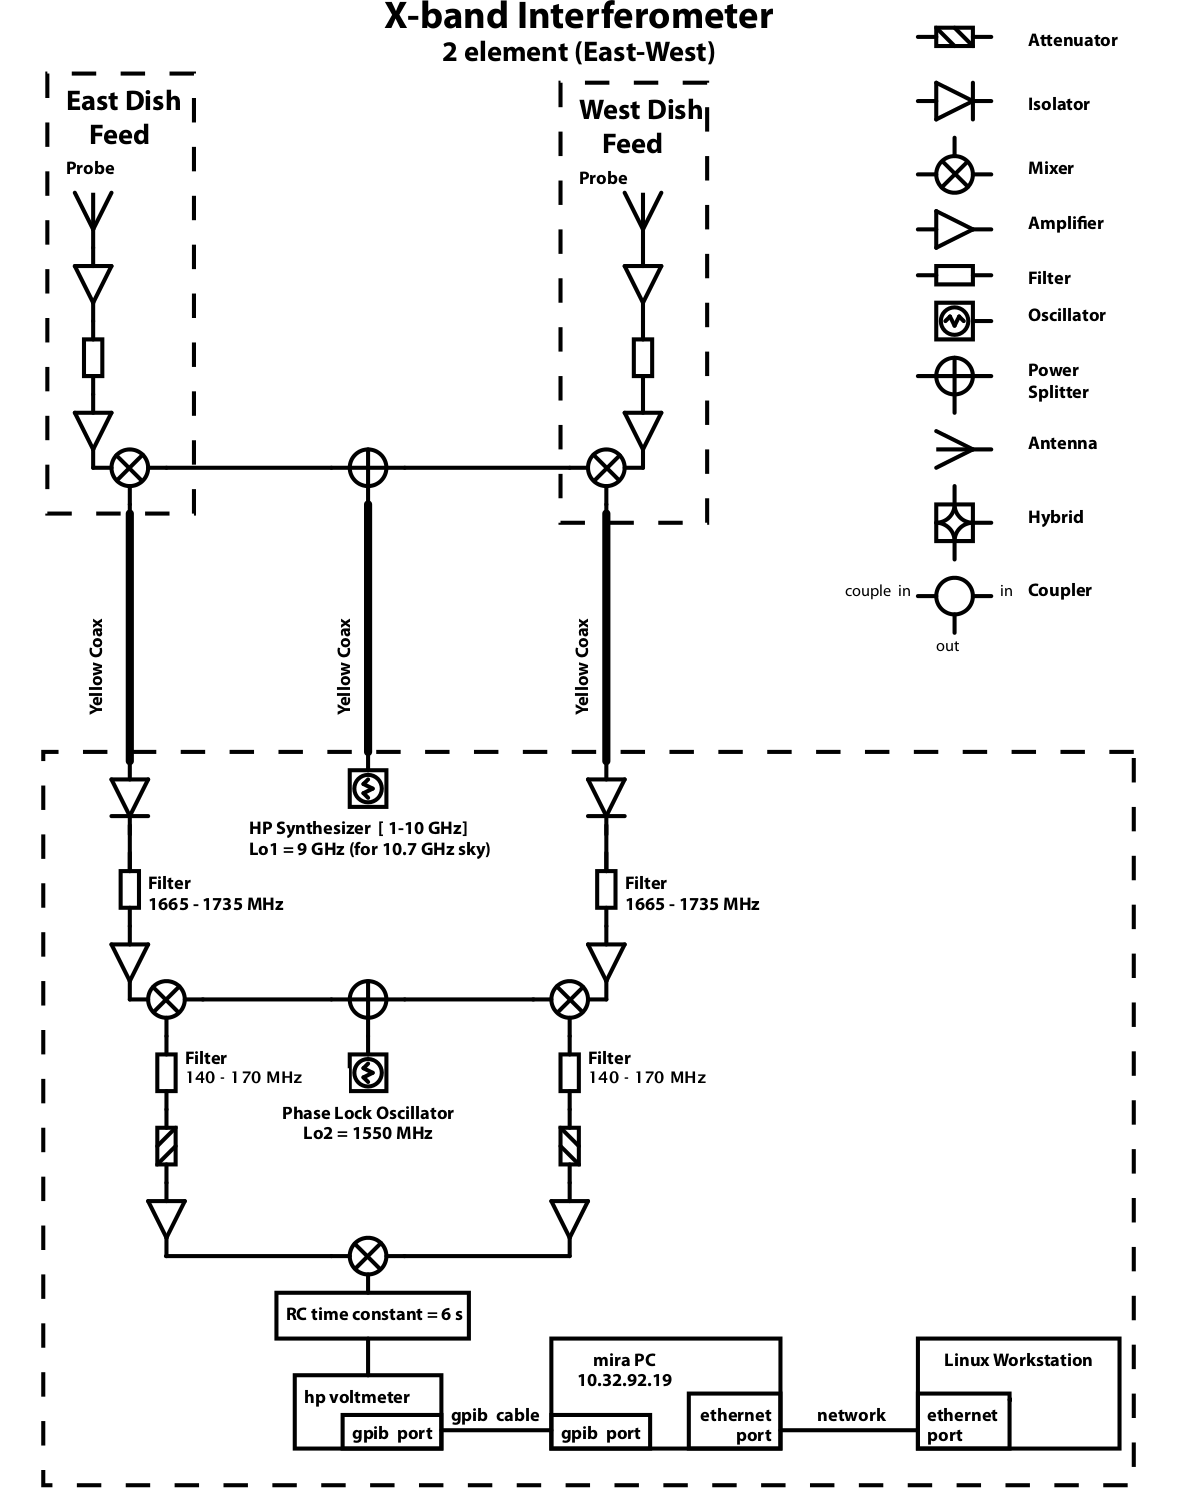
\includegraphics[scale=0.7]{img/signal_path.png}
    \caption{Time domain effects of changing the ratio between the input frequency and the sampling frequency.}
    \label{fig:signal_path}
    \end{figure}

    The interferometer is mechanically limited to an altitude range of
    $15^{\circ}$ to $87^{\circ}$.

  \subsection{Coordinates}
  In order to
  \subsubsection{Data Collection}
  \subsection{Fitting}

%=======================================================================================

\section{Results \& Discussion}
  \subsection{Sampling and Aliasing}

  \subsection{Digital Mixing on an FPGA}
%=======================================================================================

\section{Conclusion}

Code and results are available online at: https://github.com/viyer/astro121

\bibliographystyle{plain}
\bibliography{references}
\end{document}
